
\documentclass[12pt]{article}

\usepackage[utf8]{inputenc}
\usepackage[greek, english]{babel}

% Packages
\usepackage{alphabeta}
\usepackage{amsmath}
\usepackage{amsthm}
\usepackage{caption}
\usepackage{color}
\usepackage{float}
\usepackage{fullpage}
\usepackage{graphicx}
\usepackage{hyperref}
\usepackage{latexsym}
\usepackage{listings}
\usepackage{pxfonts}
\usepackage{stackrel}
\usepackage{subfig}
\usepackage{tikz}
\usepackage{titlesec}

% Commands
\newcommand{\N}{\mathbb{N}}
\newcommand{\R}{\mathbb{R}}
\newcommand{\abs}[1]{\left\lvert#1\right\rvert}
\newcommand{\code}[2]{\lstinputlisting[caption={#2}]{#1}}
\newcommand{\margin}{\hspace{4pt}}
\newcommand{\norm}[1]{\left\lVert#1\right\rVert}

% Environments
\newenvironment{matlab}
	{\begin{figure}[hp]\centering\captionsetup{justification=centering}}
	{\end{figure}}

\newenvironment{rcases}
	{\left.\begin{aligned}}
	{\end{aligned}\right\rbrace}

% Python Syntax Highlighting
\definecolor{string_color}{RGB}{0, 161, 13}
\definecolor{comment_color}{RGB}{46, 46, 46}
\definecolor{keyword_color}{RGB}{0, 112, 191}
\definecolor{background_color}{RGB}{250, 250, 250}

\lstset{
    framesep=15pt,
    xleftmargin=15pt,
    xrightmargin=15pt,
    language=Python,
    captionpos=b,
    numbers=right,
    numberstyle=\small\ttfamily,
    frame=lines,
    showspaces=false,
    showtabs=false,
    breaklines=true,
    showstringspaces=false,
    breakatwhitespace=true,
    commentstyle=\color{comment_color}\textit,
    keywordstyle=\bfseries\color{keyword_color}\textbf,
    stringstyle=\color{string_color}\textit,
    morekeywords={self, lambda, __init__, __del__, __name__, for, in, not, and, or, :},
    basicstyle=\small\ttfamily,
    tabsize=4,
    keepspaces=true,
    columns=flexible,
    backgroundcolor=\color{background_color}
}

% Links
\hypersetup{
    colorlinks=true,
    linkcolor=blue,
    filecolor=magenta,
    urlcolor=cyan,
}

% Lengths
\setlength{\parindent}{0in}
\setlength{\oddsidemargin}{0in}
\setlength{\textwidth}{6.5in}
\setlength{\textheight}{10in}
\setlength{\topmargin}{-1.0in}
\setlength{\headheight}{18pt}

\titlespacing*{\subsection}
{0pt}{5.5ex plus 1ex minus .2ex}{4.3ex plus .2ex}

\title{\hugeΥλοποίηση σε Python}
\author{Σιώρος Βασίλειος\\Ανδρινοπούλου Χριστίνα}
\date{Ιανουάριος 2020}

\begin{document}

\maketitle

\pagenumbering{gobble}

\pagebreak

\section{The Python equivalents of the Linear Programming Formulations of Sudoku Variations}

\subsection{Classic Sudoku}

\begin{lstlisting}[caption={TODO}]
self.matrix = matrix
self.n = len(matrix)
self.m = int(sqrt(self.n))

super().__init__(
    name=f"{type(self).__name__}_solver_{self.n}_x_{self.n}".lower(),
    sense=LpMinimize)
\end{lstlisting}

\begin{lstlisting}[caption={TODO}]
self.x = [
    [
        [
            LpVariable(
                f"x_{i + 1:02d}_{j + 1:02d}_{k + 1:02d}", cat=LpBinary)
            for k in range(self.n)
        ] for j in range(self.n)
    ] for i in range(self.n)
]
\end{lstlisting}

\begin{lstlisting}[caption={TODO}]
self += 0
\end{lstlisting}

\begin{lstlisting}[caption={TODO}]
    for j in range(self.n):
        for k in range(self.n):
            self += lpSum([self.x[i][j][k]
                            for i in range(self.n)]) == 1, f"in column {j + 1:02d} only one {k + 1:02d}"
\end{lstlisting}

\begin{lstlisting}[caption={TODO}]
    for i in range(self.n):
        for k in range(self.n):
            self += lpSum([self.x[i][j][k]
                            for j in range(self.n)]) == 1, f"in row {i + 1:02d} only one {k + 1:02d}"
\end{lstlisting}

\begin{lstlisting}[caption={TODO}]
    for k in range(self.n):
        for p in range(self.m):
            for q in range(self.m):
                self += lpSum([
                    [
                        lpSum([
                            self.x[i][j][k]
                            for i in range(self.m * p, self.m * (p + 1))
                        ])
                    ]
                    for j in range(self.m * q, self.m * (q + 1))
                ]) == 1, f"in submatrix {p + 1:02d} {q + 1:02d} only one {k + 1:02d}"
\end{lstlisting}

\begin{lstlisting}[caption={TODO}]
    for i in range(self.n):
        for j in range(self.n):
            self += lpSum([self.x[i][j][k]
                            for k in range(self.n)]) == 1, f"cell {i + 1:02d} {j + 1:02d} must be assigned exactly one value"
\end{lstlisting}

\begin{lstlisting}[caption={TODO}]
    for i in range(self.n):
        for j in range(self.n):
            if self.matrix[i][j]:
                self += self.x[i][j][self.matrix[i][j] -
                                        1] == 1, f"cell {i + 1:02d} {j + 1:02d} has an initial value of {self.matrix[i][j]:02d}"
\end{lstlisting}

\begin{lstlisting}[caption={TODO}]
    for i in range(self.n):
        for j in range(self.n):
            if not self.matrix[i][j]:
                for value in self.illegal_values(i, j):
                    self += (
                        self.x[i][j][value - 1] == 0,
                        f"cell {i + 1:02d} {j + 1:02d} cannot be assigned a value of {value:02d}"
                    )
\end{lstlisting}

\begin{lstlisting}[caption={TODO}]
def solve(self, solver=None, **kwargs):

    super().solve(solver=solver, **kwargs)

    if LpStatus[self.status] != "Optimal":
        raise ValueError(
            f"Solver failed with status '{LpStatus[self.status]}'")

    for i in range(self.n):
        for j in range(self.n):
            if not self.matrix[i][j]:
                self.matrix[i][j] = [
                    self.x[i][j][k].varValue for k in range(self.n)
                ].index(1) + 1
\end{lstlisting}

\begin{lstlisting}[caption={TODO}]
def illegal_values(self, row, col):

    values = set()

    for j in range(self.n):
        if self.matrix[row][j] is not None:
            values.add(self.matrix[row][j])

    for i in range(self.n):
        if self.matrix[i][col] is not None:
            values.add(self.matrix[i][col])

    p, q = row // self.m, col // self.m

    for i in range(self.m * p, self.m * (p + 1)):
        for j in range(self.m * q, self.m * (q + 1)):
            if self.matrix[i][j] is not None:
                values.add(self.matrix[i][j])

    return values
\end{lstlisting}

\begin{lstlisting}[caption={TODO}]
sudokulp_solver_9_x_9:
MINIMIZE
0*__dummy + 0
\end{lstlisting}

\begin{lstlisting}[caption={TODO}]
SUBJECT TO
in_column_01_only_one_01: x_01_01_01 + x_02_01_01 + x_03_01_01 + x_04_01_01
+ x_05_01_01 + x_06_01_01 + x_07_01_01 + x_08_01_01 + x_09_01_01 = 1
...
in_column_09_only_one_09: x_01_09_09 + x_02_09_09 + x_03_09_09 + x_04_09_09
+ x_05_09_09 + x_06_09_09 + x_07_09_09 + x_08_09_09 + x_09_09_09 = 1

in_row_01_only_one_01: x_01_01_01 + x_01_02_01 + x_01_03_01 + x_01_04_01
+ x_01_05_01 + x_01_06_01 + x_01_07_01 + x_01_08_01 + x_01_09_01 = 1
...
in_row_09_only_one_09: x_09_01_09 + x_09_02_09 + x_09_03_09 + x_09_04_09
+ x_09_05_09 + x_09_06_09 + x_09_07_09 + x_09_08_09 + x_09_09_09 = 1

in_submatrix_01_01_only_one_01: x_01_01_01 + x_01_02_01 + x_01_03_01
+ x_02_01_01 + x_02_02_01 + x_02_03_01 + x_03_01_01 + x_03_02_01 + x_03_03_01
= 1
...
in_submatrix_03_03_only_one_09: x_07_07_09 + x_07_08_09 + x_07_09_09
+ x_08_07_09 + x_08_08_09 + x_08_09_09 + x_09_07_09 + x_09_08_09 + x_09_09_09
= 1

cell_01_01_must_be_assigned_exactly_one_value: x_01_01_01 + x_01_01_02
+ x_01_01_03 + x_01_01_04 + x_01_01_05 + x_01_01_06 + x_01_01_07 + x_01_01_08
+ x_01_01_09 = 1
...
cell_09_09_must_be_assigned_exactly_one_value: x_09_09_01 + x_09_09_02
+ x_09_09_03 + x_09_09_04 + x_09_09_05 + x_09_09_06 + x_09_09_07 + x_09_09_08
+ x_09_09_09 = 1

cell_01_08_has_an_initial_value_of_02: x_01_08_02 = 1
...
cell_09_02_has_an_initial_value_of_01: x_09_02_01 = 1

cell_01_01_cannot_be_assigned_a_value_of_02: x_01_01_02 = 0
...
cell_09_09_cannot_be_assigned_a_value_of_09: x_09_09_09 = 0
\end{lstlisting}

\begin{lstlisting}[caption={TODO}]
VARIABLES
__dummy = 0 Continuous
0 <= x_01_01_01 <= 1 Integer
...
0 <= x_09_09_09 <= 1 Integer
\end{lstlisting}

\pagebreak

\subsection{Sudoku X}

\begin{lstlisting}[caption={TODO}]
super().__init__(matrix)
\end{lstlisting}

\begin{lstlisting}[caption={TODO}]
for k in range(self.n):

    self += lpSum([
        self.x[r][r][k] for r in range(self.n)
    ]) == 1, f"in the diagonal only one {k + 1}"
\end{lstlisting}

\begin{lstlisting}[caption={TODO}]
for k in range(self.n):

    self += lpSum([
        self.x[r][self.n - 1 - r][k] for r in range(self.n)
    ]) == 1, f"in the anti diagonal only one {k + 1}"
\end{lstlisting}

\pagebreak

\subsection{Four Square Sudoku}

\begin{lstlisting}[caption={TODO}]
super().__init__(matrix)
\end{lstlisting}

\begin{lstlisting}[caption={TODO}]
for i in [1, self.n - self.m - 1]:
    for j in [1, self.n - self.m - 1]:
        for k in range(self.n):
            self += lpSum([
                [
                    lpSum([
                        self.x[r][c][k]
                        for c in range(j, j + self.m)
                    ])
                ]
                for r in range(i, i + self.m)
            ]) == 1, f"in square {i + 1:02d} {j + 1:02d} {i + self.m:02d} {j + self.m:02d} only one {k + 1:02d}"
\end{lstlisting}

\pagebreak

\subsection{Four Pyramid Sudoku}

\begin{lstlisting}[caption={TODO}]
super().__init__(matrix)
\end{lstlisting}

\begin{lstlisting}[caption={TODO}]
for k in range(1, self.n + 1):
    self += lpSum([
        lpSum([
            self.x[r - 1][c - 1][k - 1]
            for c in range(self.m + r, self.n - r + 1)
        ]) for r in range(1, self.m + 1)
    ]) == 1, f"in pyramid 1 only one {k + 1}"
\end{lstlisting}

\begin{lstlisting}[caption={TODO}]
for k in range(1, self.n + 1):
    self += lpSum([
        lpSum([
            self.x[r - 1][c - 1][k - 1]
            for r in range(1 + c, self.n - self.m + 1 - c + 1)
        ]) for c in range(1, self.m + 1)
    ]) == 1, f"in pyramid 2 only one {k + 1}"
\end{lstlisting}

\begin{lstlisting}[caption={TODO}]
for k in range(1, self.n + 1):
    self += lpSum([
        lpSum([
            self.x[r - 1][c - 1][k - 1]
            for c in range(self.n + self.m - 1 - r, r - self.m + 1)
        ]) for r in range(self.n - self.m + 1, self.n + 1)
    ]) == 1, f"in pyramid 3 only one {k + 1}"
\end{lstlisting}

\begin{lstlisting}[caption={TODO}]
for k in range(1, self.n + 1):
    self += lpSum([
        lpSum([
            self.x[r - 1][c - 1][k - 1]
            for r in range(self.n + self.m + 1 - c, c - 1 + 1)
        ]) for c in range(self.n - self.m + 1, self.n + 1)
    ]) == 1, f"in pyramid 4 only one {k + 1}"
\end{lstlisting}

\begin{lstlisting}[caption={TODO}]
options = {
    "sdk": SudokuLP,
    "sdkx": SudokuXLP,
    "sdkfs": FourSquareSudokuLP,
    "sdkfp": FourPyramidSudokuLP
}

extension = path.splitext(args.load)[1][1:]

matrix = load(args.load)
problem = options[extension](matrix)
\end{lstlisting}

\section{Generating Sudoku Puzzles}

\begin{lstlisting}[caption={TODO}]
def transpose(matrix):
    return list(map(list, [*zip(*matrix)]))
\end{lstlisting}

\begin{lstlisting}[caption={TODO}]
def relabel(matrix):
    replacements = {
        original: replacement
        for original, replacement in zip(
            range(1, len(matrix) + 1),
            np.random.permutation(range(1, len(matrix) + 1))
        )
    }

    for i in range(len(matrix)):
        for j in range(len(matrix)):
            if matrix[i][j] is not None:
                matrix[i][j] = replacements[matrix[i][j]]

    return matrix
\end{lstlisting}

\begin{lstlisting}[caption={TODO}]
def reorder(matrix):
    def swap_rows(matrix):

        m = int(sqrt(len(matrix)))

        for p in range(m):
            for q in range(m):
                for r in range(m):
                    i1 = randint(m * p, m * (p + 1) - 1)
                    i2 = randint(m * p, m * (p + 1) - 1)

                    matrix[i1], matrix[i2] = matrix[i2], matrix[i1]

        return matrix

    return transpose(swap_rows(transpose(swap_rows(matrix))))
\end{lstlisting}

\begin{lstlisting}[caption={TODO}]
methods = {
    "transpose": transpose,
    "relabel": relabel,
    "reorder": reorder
}

matrix = load(args.load)
matrix = methods[args.method](matrix)

dump(matrix, args.save)
\end{lstlisting}

\section{The Sudoku (.sdk*) file format}

\begin{lstlisting}[caption={TODO}]
9
1, 1, 5
1, 2, 3
1, 5, 7
2, 1, 6
2, 4, 1
2, 5, 9
2, 6, 5
3, 2, 9
3, 3, 8
3, 8, 6
4, 1, 8
4, 5, 6
4, 9, 3
5, 1, 4
5, 4, 8
5, 6, 3
5, 9, 1
6, 1, 7
6, 5, 2
6, 9, 6
7, 2, 6
7, 7, 2
7, 8, 8
8, 4, 4
8, 5, 1
8, 6, 9
8, 9, 5
9, 5, 8
9, 8, 7
9, 9, 9
\end{lstlisting}

\begin{matlab}
    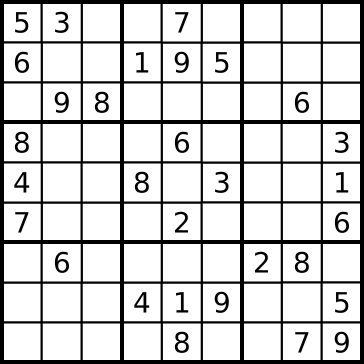
\includegraphics{figures/sudoku}
    \caption{A Sudoku Puzzle}
    \href{https://el.wikipedia.org/wiki/%CE%A3%CE%BF%CF%85%CE%BD%CF%84%CF%8C%CE%BA%CE%BF%CF%85}{Taken from Wikipedia}
\end{matlab}

\pagebreak

\subsection{Loading Sudoku Puzzles}

\begin{lstlisting}[caption={TODO}]
lines = file.readlines()
lines = map(lambda line: sub(r"#.*", "", line), lines)
lines = map(lambda line: sub(r"\s+", "", line), lines)
lines = enumerate(lines)
lines = filter(lambda data: len(data[1]) > 0, lines)
\end{lstlisting}

\begin{lstlisting}[caption={TODO}]
try:
    index, line = next(lines)

    size = int(line)

    if size <= 0:
        raise ValueError

except ValueError:
    raise ParseError(
        index, line, "is not a valid size specifier")
\end{lstlisting}

\begin{lstlisting}[caption={TODO}]
_sqrt = sqrt(size)

if _sqrt != int(_sqrt):
    raise ParseError(
        index, line, f"{size} is not a perfect square")
\end{lstlisting}

\begin{lstlisting}[caption={TODO}]
matrix = [[None for _ in range(size)] for _ in range(size)]

for index, line in lines:
    try:
        x, y, z = tuple(map(int, line.split(',')))

        if x < 0 or y < 0 or z < 0 or z > size:
            raise IndexError

        if matrix[x - 1][y - 1] is not None:
            raise ParseError(
                index, line,
                f"the cell has already been assigned")

        matrix[x - 1][y - 1] = z

    except IndexError:
        raise ParseError(
            index, line,
            f"is not a valid entry for a puzzle of size {size}")

    except ParseError as parse_error:
        raise parse_error

    except:
        raise ParseError(
            index, line, "Malformed entry")

return matrix
\end{lstlisting}

\pagebreak

\subsection{Dumping Sudoku Puzzles}

\begin{lstlisting}[caption={TODO}]
file.write(f"{len(matrix)}\n")

for i in range(len(matrix)):
    for j in range(len(matrix)):
        if matrix[i][j] is not None:
            file.write(f"{i + 1}, {j + 1}, {matrix[i][j]}\n")
\end{lstlisting}

\end{document}
